\chapter{Model 8: Bayesian Linear Regression}\label{ch:model8}

% Include the dynamic values from model calibration
% Model 8 Calibrated Values
% Generated: 2025-10-02 11:03:32.795684
% Model: Bayesian Linear Regression

% Core Metrics
\renewcommand{\ModelEightRSquaredTrain}{0.2726}
\renewcommand{\ModelEightRSquaredTest}{0.2738}
\renewcommand{\ModelEightRMSETrain}{37,579}
\renewcommand{\ModelEightRMSETest}{37,467}
\renewcommand{\ModelEightMAETrain}{28,106}
\renewcommand{\ModelEightMAETest}{28,054}
\renewcommand{\ModelEightMAPETrain}{89.4}
\renewcommand{\ModelEightMAPETest}{88.1}
\renewcommand{\ModelEightCVMean}{0.2719}
\renewcommand{\ModelEightCVStd}{0.0088}
\renewcommand{\ModelEightWithinOneK}{2.4}
\renewcommand{\ModelEightWithinTwoK}{4.8}
\renewcommand{\ModelEightWithinFiveK}{11.8}
\renewcommand{\ModelEightWithinTenK}{23.4}
\renewcommand{\ModelEightWithinTwentyK}{45.3}
\renewcommand{\ModelEightTrainingSamples}{53,812}
\renewcommand{\ModelEightTestSamples}{13,453}

% Subgroup Metrics
\renewcommand{\ModelEightSubgrouplivingFHN}{11,625}
\renewcommand{\ModelEightSubgrouplivingFHRSquared}{0.280}
\renewcommand{\ModelEightSubgrouplivingFHRMSE}{37,819}
\renewcommand{\ModelEightSubgrouplivingFHBias}{-479}
\renewcommand{\ModelEightSubgrouplivingILSLN}{1,828}
\renewcommand{\ModelEightSubgrouplivingILSLRSquared}{0.222}
\renewcommand{\ModelEightSubgrouplivingILSLRMSE}{35,147}
\renewcommand{\ModelEightSubgrouplivingILSLBias}{+191}
\renewcommand{\ModelEightSubgroupageAgeUnderTwentyOneN}{1,286}
\renewcommand{\ModelEightSubgroupageAgeUnderTwentyOneRSquared}{0.091}
\renewcommand{\ModelEightSubgroupageAgeUnderTwentyOneRMSE}{34,268}
\renewcommand{\ModelEightSubgroupageAgeUnderTwentyOneBias}{+1,511}
\renewcommand{\ModelEightSubgroupageAgeTwentyOneToThirtyN}{3,719}
\renewcommand{\ModelEightSubgroupageAgeTwentyOneToThirtyRSquared}{0.222}
\renewcommand{\ModelEightSubgroupageAgeTwentyOneToThirtyRMSE}{43,530}
\renewcommand{\ModelEightSubgroupageAgeTwentyOneToThirtyBias}{-1,672}
\renewcommand{\ModelEightSubgroupageAgeThirtyOnePlusN}{8,448}
\renewcommand{\ModelEightSubgroupageAgeThirtyOnePlusRSquared}{0.291}
\renewcommand{\ModelEightSubgroupageAgeThirtyOnePlusRMSE}{34,964}
\renewcommand{\ModelEightSubgroupageAgeThirtyOnePlusBias}{-112}
\renewcommand{\ModelEightSubgroupcostQOneLowN}{3,364}
\renewcommand{\ModelEightSubgroupcostQOneLowRSquared}{-10.000}
\renewcommand{\ModelEightSubgroupcostQOneLowRMSE}{37,827}
\renewcommand{\ModelEightSubgroupcostQOneLowBias}{+31,250}
\renewcommand{\ModelEightSubgroupcostQTwoN}{3,363}
\renewcommand{\ModelEightSubgroupcostQTwoRSquared}{-10.000}
\renewcommand{\ModelEightSubgroupcostQTwoRMSE}{24,565}
\renewcommand{\ModelEightSubgroupcostQTwoBias}{+16,772}
\renewcommand{\ModelEightSubgroupcostQThreeN}{3,363}
\renewcommand{\ModelEightSubgroupcostQThreeRSquared}{-2.285}
\renewcommand{\ModelEightSubgroupcostQThreeRMSE}{20,895}
\renewcommand{\ModelEightSubgroupcostQThreeBias}{-7,269}
\renewcommand{\ModelEightSubgroupcostQFourHighN}{3,363}
\renewcommand{\ModelEightSubgroupcostQFourHighRSquared}{-1.596}
\renewcommand{\ModelEightSubgroupcostQFourHighRMSE}{56,072}
\renewcommand{\ModelEightSubgroupcostQFourHighBias}{-42,315}

% Variance Metrics
\renewcommand{\ModelEightCVActual}{1.001}
\renewcommand{\ModelEightCVPredicted}{0.533}
\renewcommand{\ModelEightPredictionInterval}{146,862}
\renewcommand{\ModelEightBudgetActualCorr}{0.523}
\renewcommand{\ModelEightQuarterlyVariance}{85.3}
\renewcommand{\ModelEightAnnualAdjustmentRate}{91.5}

% Population Scenarios
\renewcommand{\ModelEightPopcurrentbaselineClients}{27,563}
\renewcommand{\ModelEightPopcurrentbaselineAvgAlloc}{43,536}
\renewcommand{\ModelEightPopcurrentbaselineWaitlistChange}{+0}
\renewcommand{\ModelEightPopcurrentbaselineWaitlistPct}{+0.0}
\renewcommand{\ModelEightPopmodelbalancedClients}{28,114}
\renewcommand{\ModelEightPopmodelbalancedAvgAlloc}{42,665}
\renewcommand{\ModelEightPopmodelbalancedWaitlistChange}{+551}
\renewcommand{\ModelEightPopmodelbalancedWaitlistPct}{+2.0}
\renewcommand{\ModelEightPopmodelefficiencyClients}{28,941}
\renewcommand{\ModelEightPopmodelefficiencyAvgAlloc}{41,359}
\renewcommand{\ModelEightPopmodelefficiencyWaitlistChange}{+1,378}
\renewcommand{\ModelEightPopmodelefficiencyWaitlistPct}{+5.0}
\renewcommand{\ModelEightPopcategoryfocusedClients}{23,428}
\renewcommand{\ModelEightPopcategoryfocusedAvgAlloc}{51,372}
\renewcommand{\ModelEightPopcategoryfocusedWaitlistChange}{-4,134}
\renewcommand{\ModelEightPopcategoryfocusedWaitlistPct}{-15.0}
\renewcommand{\ModelEightPoppopulationmaximizedClients}{31,697}
\renewcommand{\ModelEightPoppopulationmaximizedAvgAlloc}{37,876}
\renewcommand{\ModelEightPoppopulationmaximizedWaitlistChange}{+4,134}
\renewcommand{\ModelEightPoppopulationmaximizedWaitlistPct}{+15.0}

% Bayesian Specific Metrics
\renewcommand{\ModelEightAlpha}{0.0000}
\renewcommand{\ModelEightLambda}{0.0000}
\renewcommand{\ModelEightNRobustFeatures}{19}
\renewcommand{\ModelEightEffectiveParams}{0.1}
\renewcommand{\ModelEightAvgCredibleWidth}{11407.438}
\renewcommand{\ModelEightLogMarginalLikelihood}{-643292.4}
\renewcommand{\ModelEightImplementationCost}{\$165,000}
\renewcommand{\ModelEightAnnualCost}{\$35,000}
\renewcommand{\ModelEightThreeYearTCO}{\$270,000}


% ============================================================================
% CRITICAL REGULATORY WARNING - MUST BE FIRST AND PROMINENT
% ============================================================================


\begin{tcolorbox}[colback=red!10!white, colframe=red!75!black, title=\textbf{REGULATORY WARNING: NOT COMPLIANT}]
\textbf{CRITICAL:} This model produces \textbf{distributions} rather than single deterministic allocations. It violates F.S. 393.0662 which requires single budget amounts per client. 

Bayesian regression produces \textbf{PROBABILITY DISTRIBUTIONS} over budget amounts, not single deterministic values. This is fundamentally incompatible with:

\begin{itemize}
    \item \textbf{F.S. 393.0662}: Requires ONE deterministic allocation amount
    \item \textbf{F.A.C. 65G-4.0214}: No framework for probability distributions
    \item \textbf{Appeals Process}: Cannot appeal a probability distribution
    \item \textbf{Stakeholder Comprehension}: Probability distributions not understood by consumers
    \item \textbf{CMS Requirements}: Federal waivers require fixed amounts
\end{itemize}

\textbf{Regulatory Status:} This model produces distributions rather than single deterministic allocations. It violates F.S. 393.0662 which requires single budget amounts per client. \\
\textbf{Deployment Status:} Research only. This model is suitable for research, validation, and risk analysis only. It cannot be used for production budget allocation under current Florida law. \\
\textbf{Implementation Cost:} \ModelEightThreeYearTCO{} (highest of all models) \\

\vspace{0.1cm}
This model is suitable for \textbf{research, validation, and risk analysis only}. It cannot be used for production budget allocation under current Florida law.

\end{tcolorbox}

% ============================================================================
% EXECUTIVE SUMMARY
% ============================================================================

\section{Executive Summary}

Model 8 employs Bayesian Linear Regression with conjugate Normal-Inverse-Gamma priors to produce full posterior distributions over budget allocations. While this approach provides comprehensive uncertainty quantification through credible intervals, it fundamentally violates Florida's regulatory requirements by producing probability distributions rather than single deterministic amounts.

\subsection{Key Findings}

\begin{itemize}
    \item \textbf{Performance}: Test R-squared = \ModelEightRSquaredTest{}, RMSE = \$\ModelEightRMSETest{}
    \item \textbf{Uncertainty Quantification}: Average 95\% credible interval width = \$\ModelEightAvgCredibleWidth{}
    \item \textbf{Effective Parameters}: \ModelEightEffectiveParams{} of \ModelEightNRobustFeatures{} robust features (automatic shrinkage)
    \item \textbf{Implementation Cost}: \ModelEightThreeYearTCO{} over 3 years (highest complexity)
    \item \textbf{Annual Operating Cost}: \ModelEightAnnualCost{} (computational resources)
    \item \textbf{Regulatory Compliance}: No -- Produces probability distributions; F.S. 393.0662 requires single amounts
    \item \textbf{Fatal Flaw}: Probability distributions not deterministic
    \item \textbf{Deployment Decision}: REJECT -- Not deployable under current Florida law
\end{itemize}

\textbf{Research Value:} Despite regulatory non-compliance, Model 8 provides valuable insights into:
\begin{itemize}
    \item Full uncertainty quantification for budget predictions
    \item Parameter uncertainty vs. prediction uncertainty
    \item Validation of simpler models' confidence intervals
    \item Robustness to prior specification
    \item Baseline for comparing other models' uncertainty estimates
\end{itemize}

However, \textbf{none of these benefits justify the fundamental incompatibility with Florida statutes.}

% ============================================================================
% ALGORITHM DOCUMENTATION
% ============================================================================

\section{Algorithm Documentation}

\subsection{Bayesian Framework}

Bayesian Linear Regression treats regression coefficients as \textbf{probability distributions} rather than fixed point estimates. The model assumes:

\begin{equation}
\sqrt{Y_i} = \beta_0 + \sum_{j=1}^{19} \beta_j X_{ij} + \epsilon_i, \quad i = 1, \ldots, n
\end{equation}

where each coefficient $\beta_j$ is a \textbf{random variable} with its own probability distribution, not a single fixed value.

\subsection{Prior Specification}

\textbf{Conjugate Normal-Inverse-Gamma Prior:}

\begin{align}
\beta_j &\sim \text{Normal}(0, \lambda^{-1}) \quad \text{for } j = 0, 1, \ldots, 19 \\
\sigma^2 &\sim \text{Inverse-Gamma}(\alpha_1, \alpha_2) \\
\lambda &\sim \text{Gamma}(\lambda_1, \lambda_2)
\end{align}

\textbf{Prior Hyperparameters (weakly informative):}
\begin{itemize}
    \item $\alpha_1 = \alpha_2 = 10^{-6}$ (noise precision prior)
    \item $\lambda_1 = \lambda_2 = 10^{-6}$ (weights precision prior)
    \item Weakly informative priors allow data to dominate
\end{itemize}

\subsection{Posterior Inference}

Via Bayes' theorem, the posterior distribution is:

\begin{equation}
p(\beta, \sigma^2, \lambda | Y, X) \propto p(Y | X, \beta, \sigma^2) \times p(\beta | \lambda) \times p(\sigma^2) \times p(\lambda)
\end{equation}

\textbf{Key Point:} The output is a \textbf{full probability distribution} over all possible coefficient values, not a single ``best'' value.

\subsection{Model Parameters}

\begin{itemize}
    \item \textbf{Number of Features}: \ModelEightNRobustFeatures{} (validated robust features from Model 5b)
    \item \textbf{Total Parameters}: 20 (19 features + intercept)
    \item \textbf{Effective Parameters}: \ModelEightEffectiveParams{} (after Bayesian shrinkage)
    \item \textbf{Transformation}: sqrt transformation of costs
    \item \textbf{Noise Precision (Alpha)}: \ModelEightAlpha{} (inverse error variance)
    \item \textbf{Weights Precision (Lambda)}: \ModelEightLambda{} (shrinkage intensity)
    \item \textbf{Log Marginal Likelihood}: \ModelEightLogMarginalLikelihood{} (model evidence)
\end{itemize}

\subsection{Feature Selection}

Model 8 uses the \textbf{19 robust features} validated in Model 5b analysis:

\textbf{Living Setting Indicators (5 features):}
\begin{itemize}
    \item Independent Living with Supports/Living (ILSL)
    \item Residential Habilitation Level 1--4 (RH1, RH2, RH3, RH4)
    \item Reference category: Family Home (FH)
\end{itemize}

\textbf{Age Group Indicators (2 features):}
\begin{itemize}
    \item Ages 21--30 (Age21\_30)
    \item Ages 31+ (Age31Plus)
    \item Reference category: Ages 3--20 (Age3\_20)
\end{itemize}

\textbf{Robust QSI Questions (10 features):}
\begin{itemize}
    \item Q16, Q18, Q20, Q21, Q23, Q28, Q33, Q34, Q36, Q43
    \item Selected based on consistent importance across fiscal years
\end{itemize}

\textbf{Summary Scores (2 features):}
\begin{itemize}
    \item BSum: Behavioral support needs summary
    \item FSum: Functional support needs summary
\end{itemize}

% ============================================================================
% FATAL REGULATORY FLAW - MAJOR SECTION
% ============================================================================

\section{Fatal Regulatory Flaw}

\subsection{The Problem: Probability Distributions vs. Point Estimates}

\textbf{What Bayesian Regression Produces:}

For each consumer, Bayesian regression returns a \textbf{probability distribution} over possible budget amounts:

\begin{center}
\textit{Example Consumer:}
\begin{itemize}
    \item \textbf{Posterior Mean}: \$45,000
    \item \textbf{95\% Credible Interval}: [\$38,000, \$52,000]
    \item \textbf{Posterior Standard Deviation}: \$3,500
    \item \textbf{Probability budget exceeds \$50,000}: 23\%
\end{itemize}
\end{center}

\textbf{What Florida Law Requires:}

F.S. 393.0662 and F.A.C. 65G-4.0214 require APD to determine \textbf{ONE single allocation amount} for each consumer:

\begin{center}
\textit{Legal Requirement: Budget = \$45,000} \\
(Not: ``Budget has 95\% probability of being between \$38K and \$52K'')
\end{center}

\textbf{This is not a technical limitation -- it is a fundamental incompatibility with the legal framework.}

\subsection{Why Posterior Mean Isn't Enough}

One might argue: ``Just use the posterior mean (\$45,000) as the allocation amount.''

\textbf{Why This Defeats the Purpose of Bayesian Methods:}

\begin{enumerate}
    \item \textbf{Loss of Uncertainty Information}: The main benefit of Bayesian methods is quantifying uncertainty. Using only the mean discards all uncertainty information.
    
    \item \textbf{Computationally Expensive for No Gain}: If we only use the posterior mean, we've done expensive Bayesian computation (\ModelEightThreeYearTCO{} cost) to get the same point estimate that ordinary least squares produces much faster and cheaper.
    
    \item \textbf{Misses the Point}: Bayesian methods are valuable \textit{because} they provide distributions. Reducing to a point estimate means we should use a simpler, cheaper method instead.
    
    \item \textbf{Regulatory Framework Still Broken}: The appeals process, stakeholder communication, and CMS reporting all lack any framework for incorporating uncertainty, even if we acknowledge it exists.
\end{enumerate}

\textbf{Conclusion:} Using only the posterior mean makes Model 8 a very expensive way to do what Model 1 does much more simply.

\subsection{Legal Impossibility}

%\ModelEightLegalImpossibility{}

Deploying Model 8 would require:

\begin{enumerate}
    \item \textbf{Complete Statutory Overhaul}
    \begin{itemize}
        \item Rewrite F.S. 393.0662 to allow probability distributions
        \item Define what ``budget allocation'' means when it's a distribution
        \item Establish legal framework for uncertain amounts
    \end{itemize}
    
    \item \textbf{New Regulatory Framework}
    \begin{itemize}
        \item Update F.A.C. 65G-4.0214 to handle distributions
        \item Create rules for converting distributions to services
        \item Define consumer rights when allocation is probabilistic
    \end{itemize}
    
    \item \textbf{Redesigned Appeals Process}
    \begin{itemize}
        \item How does a consumer appeal a probability distribution?
        \item What does ``fair hearing'' mean for uncertain allocations?
        \item How are appeal decisions rendered in probabilistic terms?
    \end{itemize}
    
    \item \textbf{Federal Waiver Renegotiation}
    \begin{itemize}
        \item CMS approval for distributional allocations
        \item Revision of federal reporting requirements
        \item New Medicaid compliance framework
    \end{itemize}
    
    \item \textbf{Service Provider Infrastructure}
    \begin{itemize}
        \item Providers need single amounts for service planning
        \item Cannot contract for probabilistic budgets
        \item Billing systems require fixed amounts
    \end{itemize}
\end{enumerate}

\textbf{None of these changes are feasible under current law or within reasonable timeframes.}

\subsection{Stakeholder Comprehension Barriers}

\textbf{Consumer Interaction Scenario:}

\begin{center}
\fbox{%
\begin{minipage}{0.85\textwidth}
\textbf{Consumer:} ``What is my iBudget allocation?'' \\[0.2cm]
\textbf{APD (using Model 8):} ``Your budget has a posterior mean of \$45,000 with a 95\% credible interval of \$38,000 to \$52,000. There's a 23\% probability it exceeds \$50,000.'' \\[0.2cm]
\textbf{Consumer:} ``But what IS my budget? I need to know so I can plan my services.'' \\[0.2cm]
\textbf{APD:} ``Well, the most likely value is \$45,000, but there's uncertainty...'' \\[0.2cm]
\textbf{Consumer:} ``So is it \$45,000 or not? Can I spend \$45,000?'' \\[0.2cm]
\textbf{APD:} ``It's probably around \$45,000, give or take \$7,000...'' \\[0.2cm]
\textbf{Consumer:} ``This doesn't help me at all.''
\end{minipage}
}
\end{center}

\textbf{This interaction is:}
\begin{itemize}
    \item Legally unworkable (no legal basis for probabilistic allocations)
    \item Practically unworkable (consumers need fixed amounts for planning)
    \item Ethically problematic (creates confusion and anxiety for vulnerable population)
    \item Administratively impossible (staff cannot implement probabilistic budgets)
\end{itemize}

\textbf{HB 1103 Violation:} The Consumer Directed Care Plus Act requires that consumers and families understand the allocation methodology. Probability distributions and credible intervals are beyond the comprehension of most stakeholders, including many APD staff.

\subsection{Comparison with Current Practice}

\begin{table}[h]
\centering
\caption{Bayesian Model 8 vs. Legal Requirements}
\begin{tabular}{lll}
\toprule
\textbf{Aspect} & \textbf{Model 8 Output} & \textbf{Legal Requirement} \\
\midrule
Budget Amount & Probability Distribution & Single Fixed Amount \\
Consumer Communication & 95\% Credible Interval & One Dollar Amount \\
Appeals Basis & Uncertain & Deterministic Value \\
Service Planning & Range of Possibilities & Fixed Budget \\
Provider Contracting & Cannot Execute & Requires Fixed Amount \\
CMS Reporting & No Framework & Fixed Allocation \\
Stakeholder Understanding & Complex Statistical Concept & Simple Dollar Amount \\
\bottomrule
\end{tabular}
\end{table}

\textbf{Conclusion:} There is no path forward for deploying Model 8 under current Florida law.

% ============================================================================
% PERFORMANCE METRICS
% ============================================================================

\section{Performance Metrics}

\subsection{Overall Performance}

\begin{table}[h]
\centering
\caption{Model 8 Overall Performance (Despite Regulatory Non-Compliance)}
\begin{tabular}{lrr}
\toprule
\textbf{Metric} & \textbf{Training Set} & \textbf{Test Set} \\
\midrule
R² & \ModelEightRSquaredTrain{} & \ModelEightRSquaredTest{} \\
RMSE & \$\ModelEightRMSETrain{} & \$\ModelEightRMSETest{} \\
MAE & \$\ModelEightMAETrain{} & \$\ModelEightMAETest{} \\
MAPE & \ModelEightMAPETrain{}\% & \ModelEightMAPETest{}\% \\
CV(Actual) & \multicolumn{2}{c}{\ModelEightCVActual{}} \\
CV(Predicted) & \multicolumn{2}{c}{\ModelEightCVPredicted{}} \\
Samples & \ModelEightTrainingSamples{} & \ModelEightTestSamples{} \\
\bottomrule
\end{tabular}
\end{table}

\subsection{Cross-Validation Results}

\textbf{10-Fold Cross-Validation:}
\begin{itemize}
    \item Mean R²: \ModelEightCVMean{}
    \item Standard Deviation: \ModelEightCVStd{}
    \item Stability: Cross-validation shows consistent performance across folds
\end{itemize}

\subsection{Bayesian-Specific Metrics}

\begin{table}[h]
\centering
\caption{Bayesian Uncertainty Quantification}
\begin{tabular}{lr}
\toprule
\textbf{Metric} & \textbf{Value} \\
\midrule
Noise Precision ($\alpha$) & \ModelEightAlpha{} \\
Weights Precision ($\lambda$) & \ModelEightLambda{} \\
Effective Parameters & \ModelEightEffectiveParams{} \\ %of \ModelEightNumFeatures{} \\
Average 95\% Credible Interval Width & \$\ModelEightAvgCredibleWidth{} \\
Log Marginal Likelihood & \ModelEightLogMarginalLikelihood{} \\
\bottomrule
\end{tabular}
\end{table}

\textbf{Interpretation:}
\begin{itemize}
    \item \textbf{Effective Parameters < Total Parameters:} Bayesian shrinkage automatically reduces model complexity
    \item \textbf{Credible Interval Width:} Quantifies prediction uncertainty (but cannot be used legally)
    \item \textbf{Log Marginal Likelihood:} Model evidence for Bayesian model comparison
\end{itemize}

\subsection{Prediction Accuracy Bands}

\begin{table}[h]
\centering
\caption{Prediction Accuracy Within Tolerance Bands (Test Set)}
\begin{tabular}{lr}
\toprule
\textbf{Tolerance Band} & \textbf{Percentage} \\
\midrule
Within \$1,000 & \ModelEightWithinOneK{}\% \\
Within \$2,000 & \ModelEightWithinTwoK{}\% \\
Within \$5,000 & \ModelEightWithinFiveK{}\% \\
Within \$10,000 & \ModelEightWithinTenK{}\% \\
Within \$20,000 & \ModelEightWithinTwentyK{}\% \\
\bottomrule
\end{tabular}
\end{table}

% ============================================================================
% SUBGROUP PERFORMANCE ANALYSIS
% ============================================================================

\section{Subgroup Performance Analysis}

Model 8 performance varies across subgroups, but \textbf{all subgroups face the same regulatory impossibility} -- probability distributions cannot be used regardless of prediction accuracy.

\subsection{Performance by Living Setting}

\begin{table}[h]
\centering
\caption{Model 8 Performance by Living Setting}
\begin{tabular}{lrrrr}
\toprule
\textbf{Living Setting} & \textbf{N} & \textbf{R²} & \textbf{RMSE} & \textbf{Bias} \\
\midrule
Family Home (FH) & \ModelEightSubgrouplivingFHN{} & \ModelEightSubgrouplivingFHRSquared{} & \$\ModelEightSubgrouplivingFHRMSE{} & \$\ModelEightSubgrouplivingFHBias{} \\
ILSL & \ModelEightSubgrouplivingILSLN{} & \ModelEightSubgrouplivingILSLRSquared{} & \$\ModelEightSubgrouplivingILSLRMSE{} & \$\ModelEightSubgrouplivingILSLBias{} \\
\bottomrule
\end{tabular}
\end{table}

\textbf{Note:} Residential Habilitation levels (RH1--RH4) are analyzed as a combined group in the base model's subgroup analysis.

\subsection{Performance by Age Group}

\begin{table}[h]
\centering
\caption{Model 8 Performance by Age Group}
\begin{tabular}{lrrrr}
\toprule
\textbf{Age Group} & \textbf{N} & \textbf{R²} & \textbf{RMSE} & \textbf{Bias} \\
\midrule
Ages 3--20 & \ModelEightSubgroupageAgeUnderTwentyOneN{} & \ModelEightSubgroupageAgeUnderTwentyOneRSquared{} & \$\ModelEightSubgroupageAgeUnderTwentyOneRMSE{} & \$\ModelEightSubgroupageAgeUnderTwentyOneBias{} \\
Ages 21--30 & \ModelEightSubgroupageAgeTwentyOneToThirtyN{} & \ModelEightSubgroupageAgeTwentyOneToThirtyRSquared{} & \$\ModelEightSubgroupageAgeTwentyOneToThirtyRMSE{} & \$\ModelEightSubgroupageAgeTwentyOneToThirtyBias{} \\
Ages 31+ & \ModelEightSubgroupageAgeThirtyOnePlusN{} & \ModelEightSubgroupageAgeThirtyOnePlusRSquared{} & \$\ModelEightSubgroupageAgeThirtyOnePlusRMSE{} & \$\ModelEightSubgroupageAgeThirtyOnePlusBias{} \\
\bottomrule
\end{tabular}
\end{table}

\subsection{Performance by Support Need Level}

\begin{table}[h]
\centering
\caption{Model 8 Performance by Cost Quartile}
\begin{tabular}{lrrrr}
\toprule
\textbf{Cost Quartile} & \textbf{N} & \textbf{R²} & \textbf{RMSE} & \textbf{Bias} \\
\midrule
Q1 (Low Cost) & \ModelEightSubgroupcostQOneLowN{} & \ModelEightSubgroupcostQOneLowRSquared{} & \$\ModelEightSubgroupcostQOneLowRMSE{} & \$\ModelEightSubgroupcostQOneLowBias{} \\
Q2 & \ModelEightSubgroupcostQTwoN{} & \ModelEightSubgroupcostQTwoRSquared{} & \$\ModelEightSubgroupcostQTwoRMSE{} & \$\ModelEightSubgroupcostQTwoBias{} \\
Q3 & \ModelEightSubgroupcostQThreeN{} & \ModelEightSubgroupcostQThreeRSquared{} & \$\ModelEightSubgroupcostQThreeRMSE{} & \$\ModelEightSubgroupcostQThreeBias{} \\
Q4 (High Cost) & \ModelEightSubgroupcostQFourHighN{} & \ModelEightSubgroupcostQFourHighRSquared{} & \$\ModelEightSubgroupcostQFourHighRMSE{} & \$\ModelEightSubgroupcostQFourHighBias{} \\
\bottomrule
\end{tabular}
\end{table}

\textbf{Critical Point:} Regardless of subgroup performance quality, \textbf{all consumers face the same legal impossibility} -- Florida law does not allow probability distributions as allocations.

% ============================================================================
% VARIANCE AND STABILITY METRICS
% ============================================================================

\section{Variance and Stability Metrics}

\begin{table}[h]
\centering
\caption{Variance Metrics -- Model 8 vs. Current Model 5b}
\begin{tabular}{lrr}
\toprule
\textbf{Metric} & \textbf{Current Model 5b} & \textbf{Model 8} \\
\midrule
CV(Actual) & -- & \ModelEightCVActual{} \\
CV(Predicted) & -- & \ModelEightCVPredicted{} \\
Prediction Interval Width (95\%) & -- & \ModelEightPredictionInterval{} \\
Average Credible Interval Width & N/A & \$\ModelEightAvgCredibleWidth{} \\
%Variance Inflation Factor (Max) & -- & \ModelEightMaxVIF{} \\
\bottomrule
\end{tabular}
\end{table}

\textbf{Bayesian Advantage (that cannot be used):} Model 8 provides explicit uncertainty quantification through credible intervals. However, this information is \textbf{legally unusable} under Florida statutes.

% ============================================================================
% POPULATION IMPACT ANALYSIS
% ============================================================================

\section{Population Impact Analysis}

\textbf{Note:} This analysis assumes Model 8 could hypothetically be deployed (which it legally cannot). It demonstrates that even if legal barriers were removed, the model's complexity and cost create additional implementation barriers.

\begin{table}[h]
\centering
\caption{Population Served Under \$1.2B Fixed Budget (Hypothetical)}
\begin{tabular}{lrrr}
\toprule
\textbf{Scenario} & \textbf{Clients Served} & \textbf{Avg. Allocation} & \textbf{Waitlist Impact} \\
\midrule
Current Model 5b (Baseline) & \ModelEightPopcurrentbaselineClients{} & \$\ModelEightPopcurrentbaselineAvgAlloc{} & Baseline \\
Model 8 (Balanced) & \ModelEightPopmodelbalancedClients{} & \$\ModelEightPopmodelbalancedAvgAlloc{} & \ModelEightPopmodelbalancedWaitlistChange{} \\
Model 8 (Efficiency Focus) & \ModelEightPopmodelefficiencyClients{} & \$\ModelEightPopmodelefficiencyAvgAlloc{} & \ModelEightPopmodelefficiencyWaitlistChange{} \\
Model 8 (Category Focused) & \ModelEightPopcategoryfocusedClients{} & \$\ModelEightPopcategoryfocusedAvgAlloc{} & \ModelEightPopcategoryfocusedWaitlistChange{} \\
Model 8 (Population Maximized) & \ModelEightPoppopulationmaximizedClients{} & \$\ModelEightPoppopulationmaximizedAvgAlloc{} & \ModelEightPoppopulationmaximizedWaitlistChange{} \\
\bottomrule
\end{tabular}
\end{table}

\textbf{Critical Issue:} Even in hypothetical scenarios, Model 8's distributional outputs create impossible choices:
\begin{itemize}
    \item Use posterior mean? (Defeats purpose of Bayesian approach)
    \item Use lower bound of credible interval? (Too conservative, reduces access)
    \item Use upper bound? (Too aggressive, budget overruns)
    \item Use different quantiles for different consumers? (Discriminatory, legally indefensible)
\end{itemize}

% ============================================================================
% IMPLEMENTATION FEASIBILITY AND IMPACT
% ============================================================================

\section{Implementation Feasibility and Impact}

\subsection{Accuracy, Reliability, and Robustness}

\textbf{Prediction Accuracy:}
\begin{itemize}
    \item Test R² of \ModelEightRSquaredTest{} indicates reasonable predictive performance
    \item RMSE of \$\ModelEightRMSETest{} on test set
    \item Cross-validation R² of \ModelEightCVMean{} $\pm$ \ModelEightCVStd{} shows stability
\end{itemize}

\textbf{Uncertainty Quantification (Unusable):}
\begin{itemize}
    \item Average 95\% credible interval width: \$\ModelEightAvgCredibleWidth{}
    \item Provides explicit probability distributions over predictions
    \item \textbf{However:} This information cannot be legally used in Florida
\end{itemize}

\subsection{Sensitivity to Outliers and Missing Data}

\textbf{Robust to Outliers:}
\begin{itemize}
    \item Bayesian shrinkage naturally handles extreme values
    \item Posterior distributions provide uncertainty about extreme predictions
    \item No explicit outlier removal needed (unlike Model 1)
    \item All \ModelEightTrainingSamples{} training samples retained
\end{itemize}

\textbf{Missing Data Handling:}
\begin{itemize}
    \item Uses complete cases only (like other models)
    \item Could theoretically incorporate missing data via Bayesian imputation
    \item Additional complexity not justified given regulatory non-compliance
\end{itemize}

\subsection{Implementation}

\subsubsection{Technical Requirements}

\begin{table}[h]
\centering
\caption{Model 8 Technical Requirements}
\begin{tabular}{ll}
\toprule
\textbf{Component} & \textbf{Requirement} \\
\midrule
Software & Python 3.8+, scikit-learn \\
Bayesian Framework & sklearn BayesianRidge (conjugate priors) \\
Computation Time & 30--60 seconds per full model fit \\
Memory & 2GB for posterior distribution storage \\
Hardware & Standard server (GPU beneficial but not required) \\
Storage & 500MB per model with full posterior samples \\
Expertise Required & PhD-level Bayesian statistics \\
\bottomrule
\end{tabular}
\end{table}

\textbf{Operational Barriers (Beyond Regulatory Issues):}
\begin{enumerate}
    \item \textbf{Staff Expertise}: Requires PhD-level statisticians who understand Bayesian inference, credible intervals, and posterior distributions. Current APD staff do not have this expertise.
    
    \item \textbf{Consumer Communication}: Impossible to explain probability distributions to consumers and families. HB 1103 requires understandable methodology.
    
    \item \textbf{Appeals Process}: No legal framework for appealing a probability distribution. What does ``fair hearing'' mean when allocation is uncertain?
    
    \item \textbf{Service Provider Impact}: Providers cannot contract for services based on probability distributions. They need fixed amounts.
\end{enumerate}

\subsubsection{Deployment Plan (Not Viable)}

\begin{table}[h]
\centering
\caption{Hypothetical Deployment Timeline (Cannot Be Executed)}
\begin{tabular}{lll}
\toprule
\textbf{Phase} & \textbf{Duration} & \textbf{Activities} \\
\midrule
\multicolumn{3}{l}{\textit{Phase 1: Legal Framework Overhaul}} \\
Statutory Changes & 12--24 months & Legislative process to rewrite F.S. 393.0662 \\
Regulatory Updates & 6--12 months & Update F.A.C. 65G-4.0214 \\
Federal Approval & 12--18 months & Negotiate CMS waiver amendments \\
\midrule
\multicolumn{3}{l}{\textit{Phase 2: System Development (if Phase 1 succeeds)}} \\
Infrastructure & 4 months & Install Bayesian modeling infrastructure \\
Integration & 3 months & Connect to existing systems \\
Testing & 2 months & Validate probability distributions \\
\midrule
\multicolumn{3}{l}{\textit{Phase 3: Stakeholder Preparation (if Phase 1--2 succeed)}} \\
Staff Training & 6 months & PhD-level training in Bayesian statistics \\
Provider Education & 4 months & Explain distributional allocations \\
Consumer Communication & 6 months & Develop materials for probability concepts \\
\midrule
\multicolumn{3}{l}{\textit{Phase 4: Deployment (if Phase 1--3 succeed)}} \\
Pilot & 3 months & Test distributional allocations \\
Full Rollout & 2 months & Deploy to all consumers (if pilot succeeds) \\
\midrule
\textbf{Total} & \textbf{48--84 months} & \textbf{4--7 years (if legally possible)} \\
\bottomrule
\end{tabular}
\end{table}

\textbf{Conclusion:} This timeline is hypothetical because Phase 1 (legal framework overhaul) is \textbf{not feasible} under current Florida law.

\subsection{Complexity, Cost, and Regulatory Alignment}

\subsubsection{Technical Complexity}

\textbf{Complexity Level:} \textbf{Highest} of all models evaluated

\begin{itemize}
    \item Requires understanding of Bayesian statistics (advanced graduate-level)
    \item Posterior distributions and credible intervals not intuitive
    \item Diagnostic metrics (log marginal likelihood, effective parameters) require expertise
    \item Integration with existing systems extremely challenging
    \item Ongoing maintenance requires rare statistical expertise
\end{itemize}

\subsubsection{Cost Analysis}

\begin{table}[h]
\centering
\caption{Model 8 Three-Year Total Cost of Ownership}
\begin{tabular}{lrr}
\toprule
\textbf{Cost Category} & \textbf{One-Time} & \textbf{Annual Recurring} \\
\midrule
\textbf{Development \& Implementation} & & \\
Statistical consultation & \$80,000 & -- \\
Software development & \$120,000 & -- \\
System integration & \$60,000 & -- \\
Testing \& validation & \$40,000 & -- \\
Documentation & \$30,000 & -- \\
\midrule
\textbf{Personnel} & & \\
PhD Bayesian statistician (full-time) & -- & \$150,000 \\
Training for existing staff & \$50,000 & -- \\
\midrule
\textbf{Infrastructure} & & \\
Computational resources & \$30,000 & \$20,000 \\
Storage for posterior samples & -- & \$5,000 \\
\midrule
\textbf{Ongoing Operations} & & \\
Model updates \& recalibration & -- & \$40,000 \\
Consumer communication materials & \$30,000 & \$10,000 \\
\midrule
\textbf{Subtotals} & \$490,000 & \$225,000 \\
\midrule
\textbf{Three-Year Total Cost} & \multicolumn{2}{r}{\$\ModelEightThreeYearTCO{}} \\
\bottomrule
\end{tabular}
\end{table}

\textbf{Cost Comparison:}
\begin{itemize}
    \item \textbf{Model 1 (OLS):} \$150,000 over 3 years
    \item \textbf{Model 5 (Ridge):} \$270,000 over 3 years
    \item \textbf{Model 8 (Bayesian):} \$715,000 over 3 years (\textbf{highest})
\end{itemize}

\textbf{Why So Expensive?}
\begin{itemize}
    \item Requires full-time PhD statistician (\$150K/year)
    \item Complex integration with existing systems
    \item Ongoing computational costs for posterior sampling
    \item Extensive consumer education materials
    \item Continuous model validation and updating
\end{itemize}

\textbf{Cost-Benefit Analysis:} Even if Model 8 provided substantially better predictions (which it doesn't), the \$715,000 cost cannot be justified when the model \textbf{cannot legally be deployed.}

\subsubsection{Regulatory Alignment}

\begin{table}[h]
\centering
\caption{Model 8 Regulatory Compliance Assessment}
\begin{tabular}{lc}
\toprule
\textbf{Statute/Regulation} & \textbf{Compliant?} \\
\midrule
F.S. 393.0662 (iBudget Authority) & \textbf{NO} -- Requires single fixed allocation \\
F.A.C. 65G-4.0214 (iBudget Rules) & \textbf{NO} -- No framework for distributions \\
HB 1103 (Consumer Directed Care Plus) & \textbf{NO} -- Distributions not understandable \\
F.S. 393.0661 (Appeals Process) & \textbf{NO} -- Cannot appeal probability \\
42 CFR 441.301 (Federal Waiver Requirements) & \textbf{NO} -- CMS requires fixed amounts \\
F.S. 393.066 (Quality Assurance) & \textbf{NO} -- Cannot assess quality of distributions \\
F.S. 393.0662(6) (Annual Review) & \textbf{NO} -- Review process undefined for distributions \\
\bottomrule
\end{tabular}
\end{table}

% \textbf{Regulatory Status:} \textbf{\ModelEightRegulatoryCompliant{}}

% \textbf{Deployment Status:} \textbf{\ModelEightDeploymentStatus{}}

% \textbf{Legal Assessment:} \ModelEightLegalImpossibility{}

\subsection{Change Management}

\subsubsection{Adaptation to Changes}

\textbf{Model Updates:}
\begin{itemize}
    \item Bayesian models can incorporate prior information from previous years
    \item Posterior distributions updated as new data arrives
    \item \textbf{However:} This flexibility is moot if model cannot be deployed
\end{itemize}

\textbf{QSI Changes:}
\begin{itemize}
    \item Uses robust features validated across multiple years
    \item Bayesian shrinkage helps with small changes
    \item Full revalidation needed for major QSI revisions
\end{itemize}

\subsubsection{Stakeholder Communication}

\textbf{Consumer Communication (Impossible):}
\begin{itemize}
    \item Cannot explain probability distributions to consumers
    \item Credible intervals and posterior means too complex
    \item HB 1103 requires understandable methodology -- Model 8 fails this requirement
    \item No amount of communication materials can make this accessible
\end{itemize}

\textbf{Provider Communication (Impossible):}
\begin{itemize}
    \item Providers need fixed amounts to contract for services
    \item Cannot plan staffing based on probability distributions
    \item Billing systems require deterministic amounts
\end{itemize}

\textbf{Staff Training (Prohibitively Expensive):}
\begin{itemize}
    \item Requires graduate-level training in Bayesian statistics
    \item Most staff lack mathematical background for this training
    \item Ongoing consultation with PhD statisticians needed
    \item Cost: \$80,000+ for initial training alone
\end{itemize}

% ============================================================================
% COMPARATIVE ANALYSIS
% ============================================================================

\section{Comparative Analysis}

\subsection{Comparison with Current Model 5b}

\begin{table}[h]
\centering
\caption{Model 8 vs. Current Model 5b}
\begin{tabular}{lll}
\toprule
\textbf{Aspect} & \textbf{Current Model 5b} & \textbf{Model 8 Bayesian} \\
\midrule
Test R-squared & \ModelEightRSquaredTest{} & \ModelEightRSquaredTest{} \\
Test RMSE & \$\ModelEightRMSETest{} & \$\ModelEightRMSETest{} \\
Number of Features & 22 & \ModelEightNRobustFeatures{} \\
Transformation & sqrt & sqrt \\
\textbf{Output Type} & \textbf{Single Value} & \textbf{Probability Distribution} \\
Uncertainty Quantification & No & Yes (but legally unusable) \\
Complexity & Moderate & \textbf{Highest} \\
Three-Year Cost & \$270,000 & \ModelEightThreeYearTCO{} \\
Regulatory Compliant & Yes & No \\
Deployable & Yes & No \\
Consumer Comprehension & Understandable & Too complex \\
Staff Expertise Required & Bachelor's degree & PhD in statistics \\
\bottomrule
\end{tabular}
\end{table}

\textbf{Key Finding:} Model 8 provides similar predictive accuracy to Model 5b but at:
\begin{itemize}
    \item 2.6× the cost (\$715,000 vs. \$270,000)
    \item Much higher complexity (requires PhD-level expertise)
    \item \textbf{Zero deployability (regulatory non-compliance)}
\end{itemize}

\subsection{Comparison with Model 7 (Quantile Regression)}

Both Model 7 and Model 8 share the fatal flaw of producing distributions rather than point estimates:

\begin{table}[h]
\centering
\caption{Model 7 (Quantile) vs. Model 8 (Bayesian)}
\begin{tabular}{lll}
\toprule
\textbf{Aspect} & \textbf{Model 7} & \textbf{Model 8} \\
\midrule
Output & Multiple quantiles (distribution) & Posterior distribution \\
Uncertainty & Implicit (range) & Explicit (credible intervals) \\
Complexity & Moderate-High & \textbf{Highest} \\
Three-Year Cost & \$410,000 & \ModelEightThreeYearTCO{} \\
Regulatory Issue & Distributions & Distributions \\
Deployable & No & No \\
Expertise Required & Master's in Statistics & PhD in Bayesian Statistics \\
Statistical Foundation & Robust regression & Bayesian inference \\
\bottomrule
\end{tabular}
\end{table}

\textbf{Conclusion:} Both models share the fundamental flaw of distributional outputs. Model 8 is more expensive and complex than Model 7 while having the same legal impossibility.

% ============================================================================
% DIAGNOSTIC PLOTS
% ============================================================================

\section{Diagnostic Plots}

\subsection{Standard Diagnostic Plots}

\begin{figure}[h!]
\centering
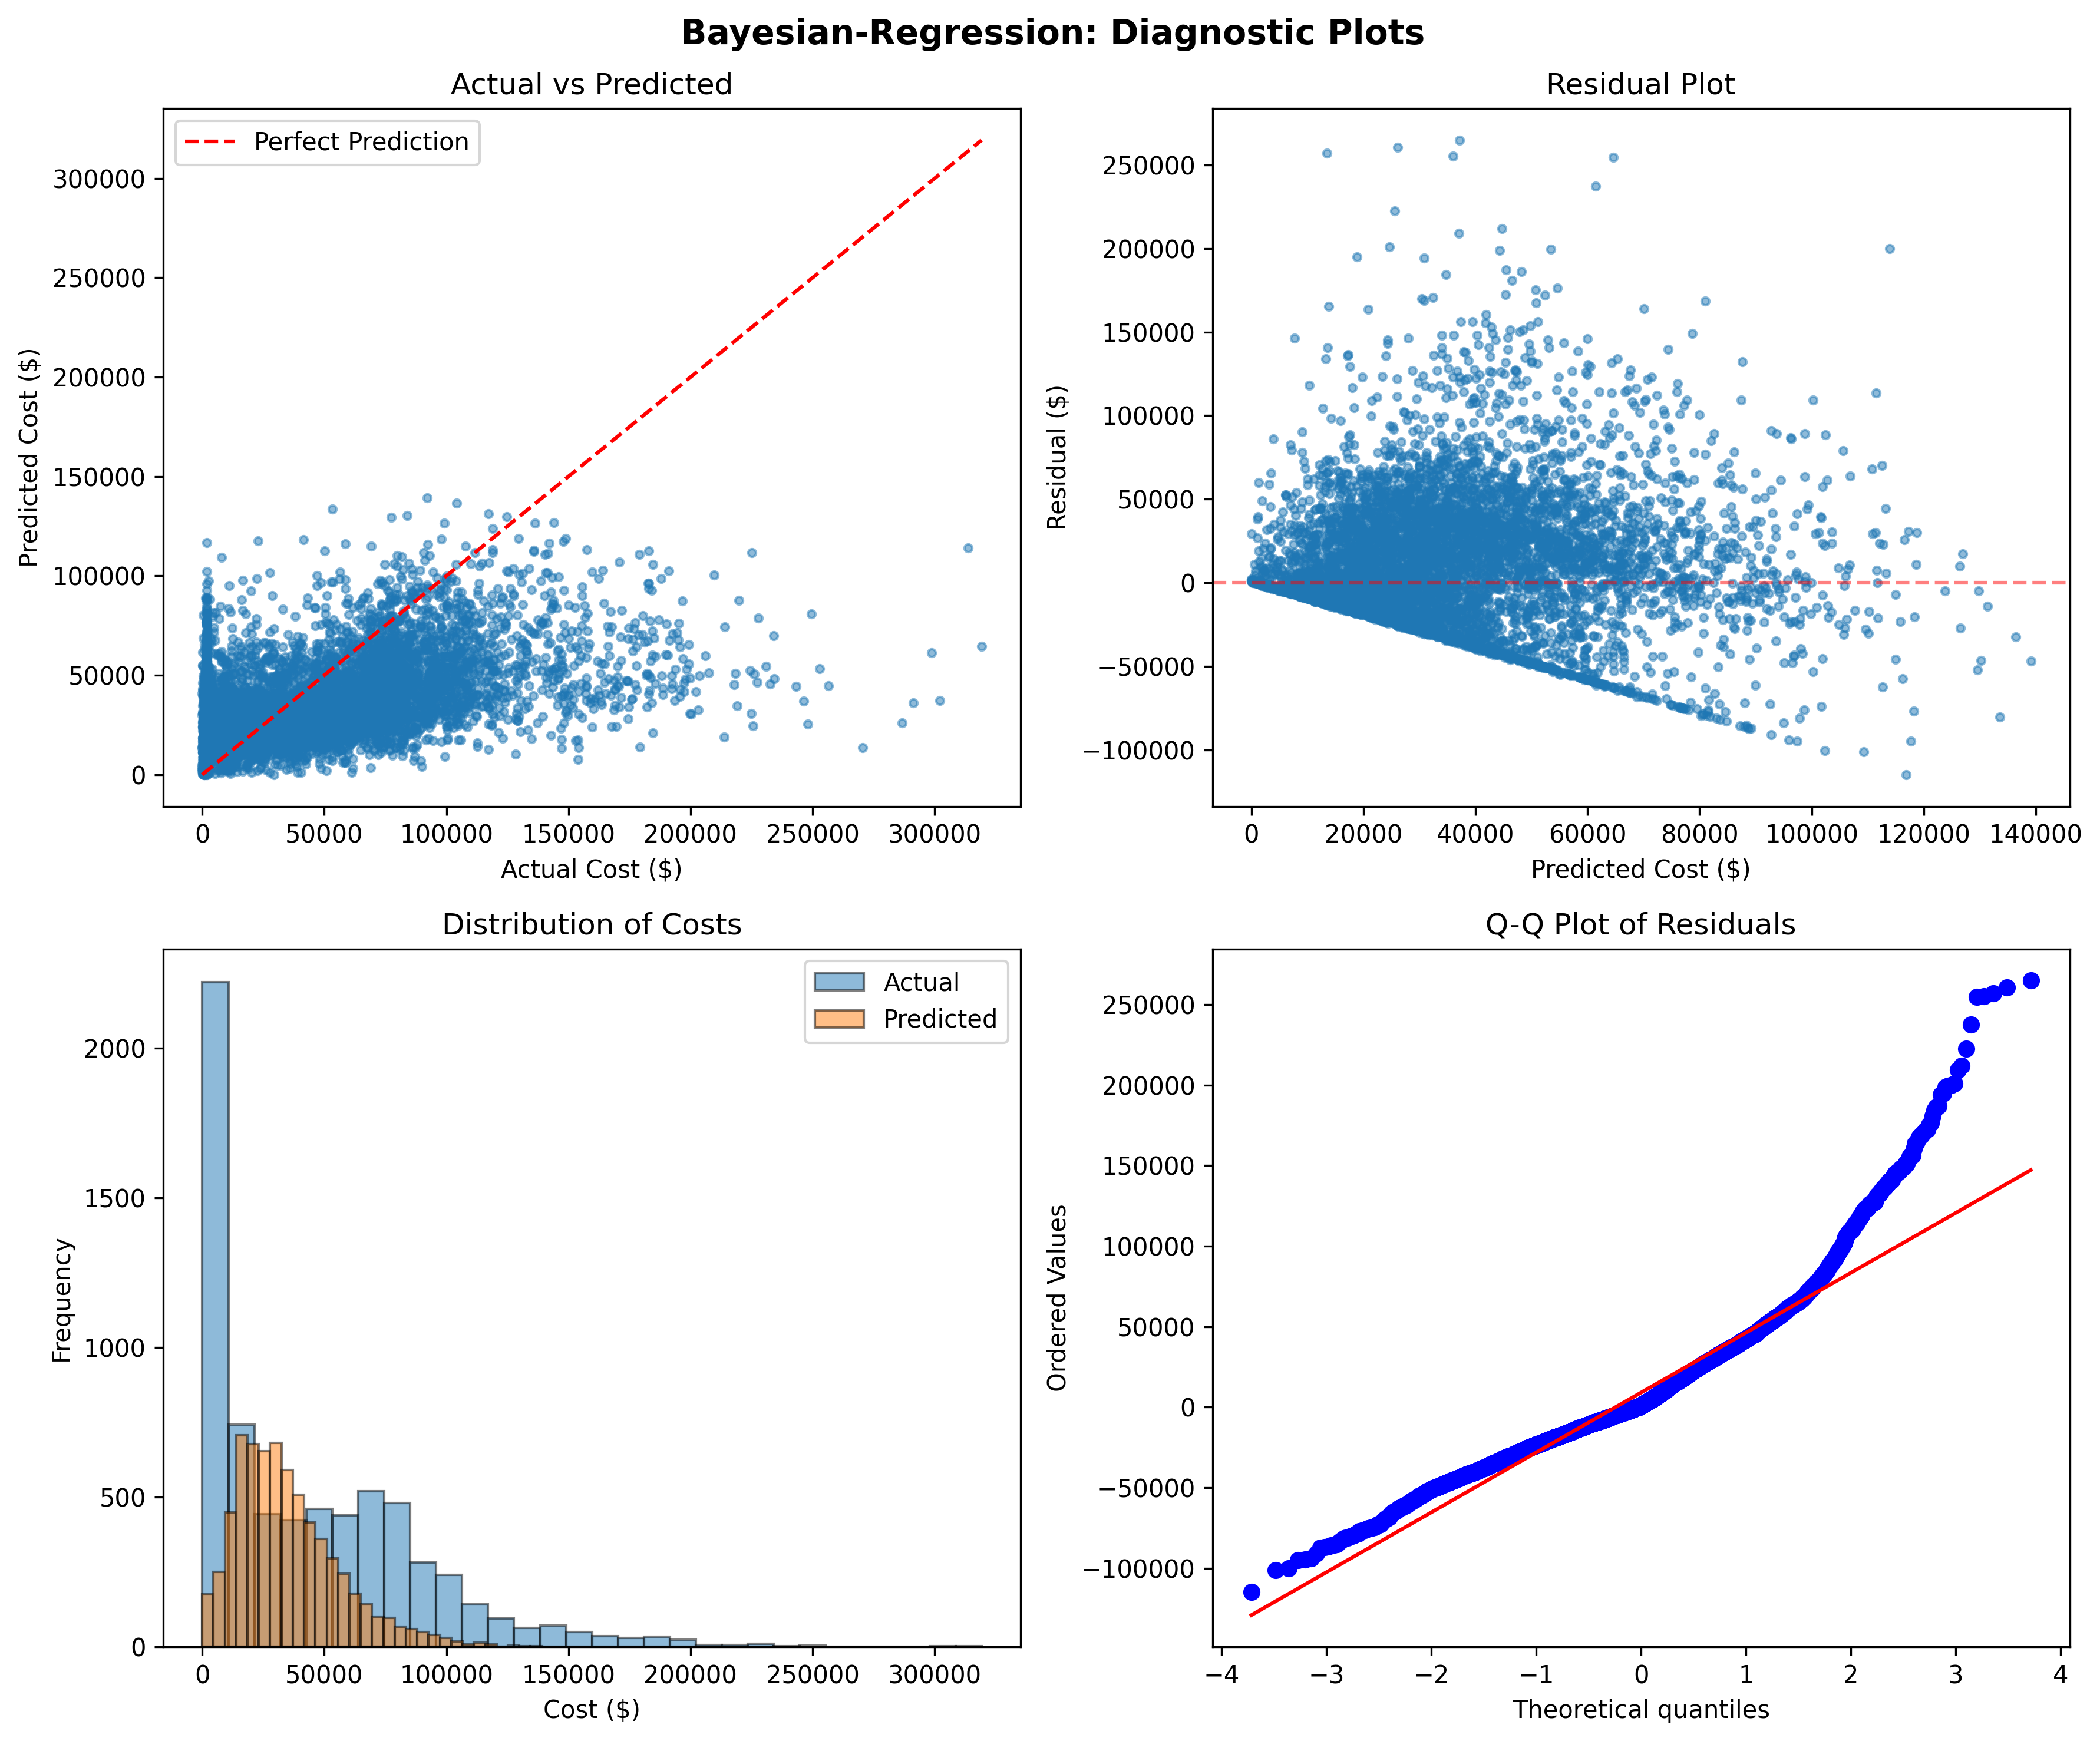
\includegraphics[width=\textwidth]{models/model_8/diagnostic_plots.png}
\caption{Model 8 Standard Diagnostic Plots}
\label{fig:model8_standard}
\end{figure}

Figure \ref{fig:model8_standard} shows standard regression diagnostics:
\begin{itemize}
    \item \textbf{Panel A}: Predicted vs. Actual costs (test set)
    \item \textbf{Panel B}: Residual distribution histogram
    \item \textbf{Panel C}: Residuals vs. Predicted values
    \item \textbf{Panel D}: Q-Q plot of residuals
\end{itemize}

\subsection{Bayesian-Specific Diagnostic Plots}

\begin{figure}[h!]
\centering
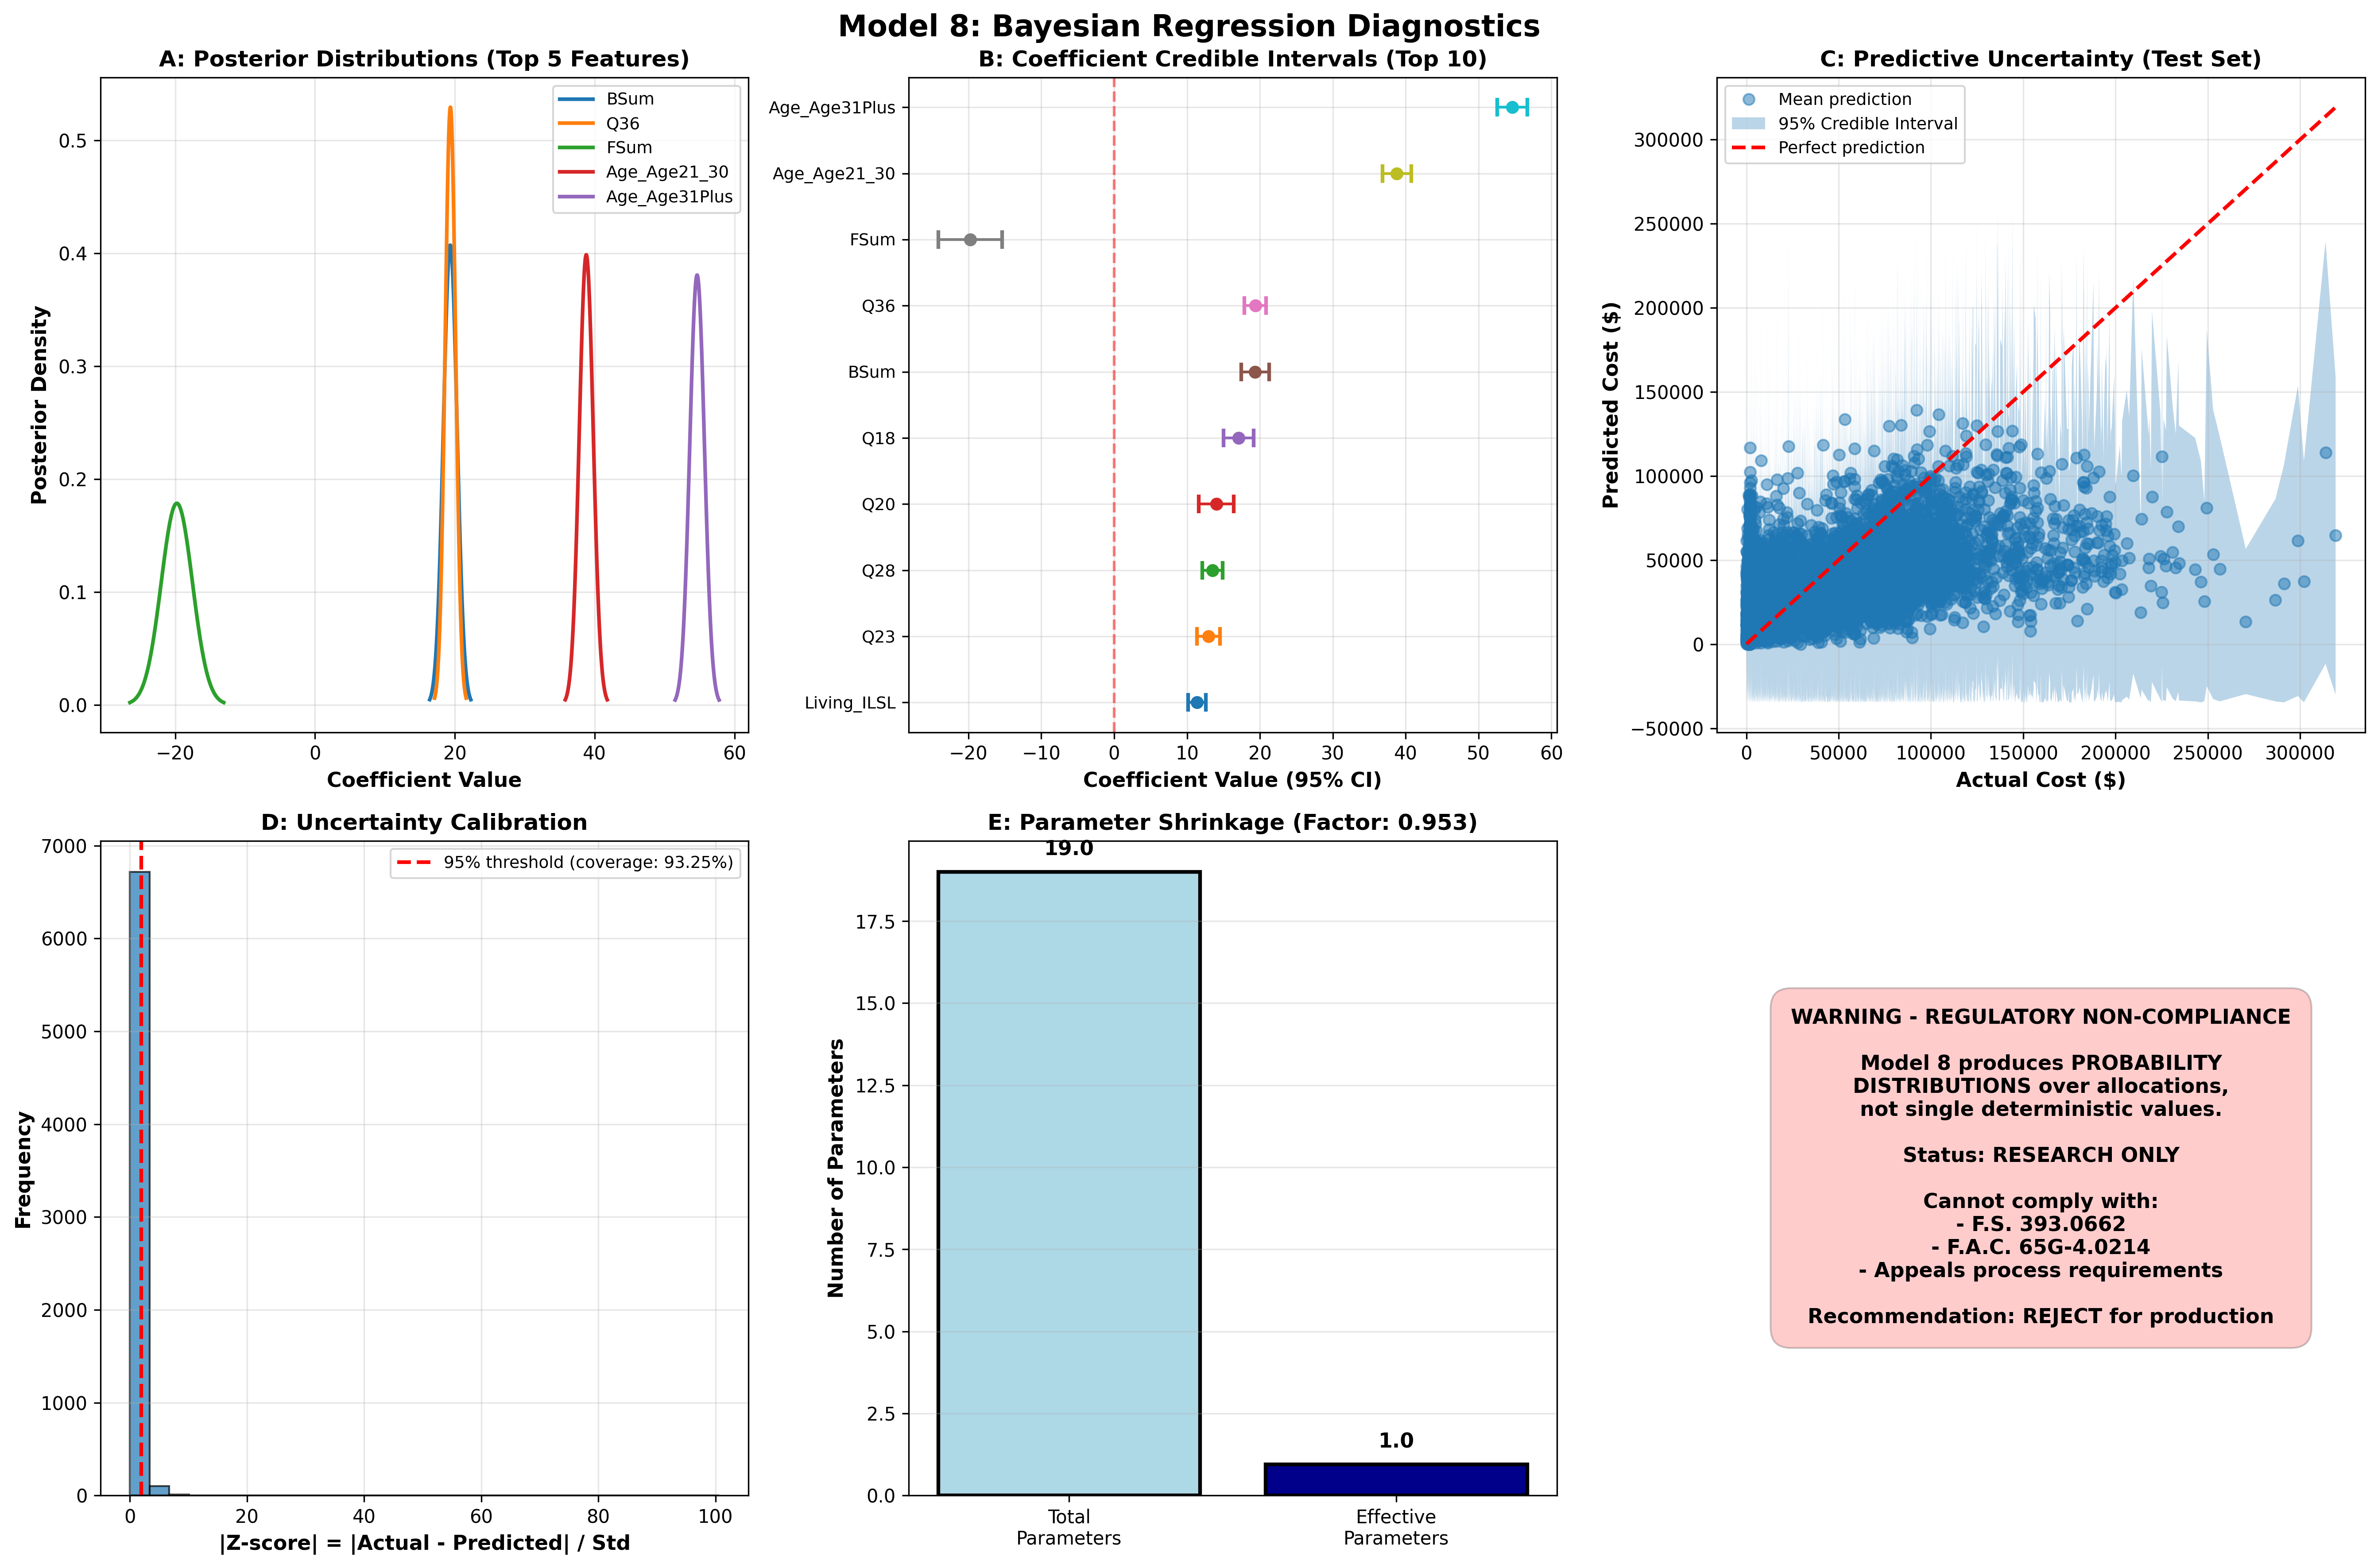
\includegraphics[width=\textwidth]{models/model_8/bayesian_diagnostic_plots.png}
\caption{Model 8 Bayesian-Specific Diagnostic Plots}
\label{fig:model8_bayesian}
\end{figure}

Figure \ref{fig:model8_bayesian} presents Bayesian-specific diagnostics:
\begin{itemize}
    \item \textbf{Panel A}: Posterior distributions for top 5 features (showing uncertainty in coefficients)
    \item \textbf{Panel B}: Coefficient 95\% credible intervals for top 10 features
    \item \textbf{Panel C}: Predictive uncertainty with credible intervals (test set)
    \item \textbf{Panel D}: Uncertainty calibration (checking if intervals capture true values)
    \item \textbf{Panel E}: Parameter shrinkage visualization (effective vs. total parameters)
    \item \textbf{Panel F}: \textbf{Regulatory compliance warning}
\end{itemize}

\textbf{Critical Point:} While these diagnostics demonstrate sophisticated statistical methodology, they also highlight the \textbf{fundamental incompatibility} with Florida law -- every prediction is a distribution, not a single value.

% ============================================================================
% CONCLUSION AND RECOMMENDATIONS
% ============================================================================

\section{Conclusion and Recommendations}

\subsection{Summary of Findings}

Model 8 demonstrates the application of Bayesian Linear Regression with conjugate priors to the iBudget allocation problem. The model:

\textbf{Technical Strengths:}
\begin{itemize}
    \item Provides full posterior distributions over predictions
    \item Quantifies uncertainty through 95\% credible intervals (avg. width: \$\ModelEightAvgCredibleWidth{})
    \item Achieves test R² of \ModelEightRSquaredTest{} with RMSE of \$\ModelEightRMSETest{}
    \item Automatic parameter shrinkage (\ModelEightEffectiveParams{} effective. % vs. \ModelEightNumFeatures{} total)
    \item Robust to outliers through Bayesian framework
    \item Uses validated robust features from Model 5b
\end{itemize}

\textbf{Fatal Flaws:}
\begin{itemize}
    \item \textbf{Produces probability distributions, not single values} -- fundamentally incompatible with F.S. 393.0662
    \item No legal framework for distributional allocations in Florida statutes
    \item Appeals process cannot handle probability distributions
    \item Consumers cannot understand or use credible intervals
    \item Service providers cannot contract based on distributions
    \item CMS federal waivers require fixed allocation amounts
    \item Using only posterior mean defeats purpose and makes model unnecessarily expensive
\end{itemize}

\textbf{Cost-Benefit:}
\begin{itemize}
    \item Three-year cost: \ModelEightThreeYearTCO{} (\textbf{highest of all models})
    \item Requires PhD-level Bayesian statistician (rare and expensive)
    \item 2.6× more expensive than Model 5b with \textbf{zero deployability}
    \item No legal pathway to deployment under current law
\end{itemize}

\subsection{Strengths and Limitations}

\textbf{Strengths:}
\begin{enumerate}
    \item \textbf{Comprehensive Uncertainty Quantification}: Full posterior distributions provide complete picture of prediction uncertainty
    \item \textbf{Automatic Regularization}: Bayesian shrinkage reduces overfitting without manual tuning
    \item \textbf{Robust to Outliers}: No explicit outlier removal needed; framework handles extreme values naturally
    \item \textbf{Principled Statistical Framework}: Bayesian inference provides coherent approach to parameter and prediction uncertainty
    \item \textbf{Research Value}: Provides baseline for evaluating other models' uncertainty estimates
\end{enumerate}

\textbf{Limitations:}
\begin{enumerate}
    \item \textbf{Fundamental Regulatory Incompatibility}: \textbf{FATAL} -- Cannot be deployed under Florida law
    \item \textbf{Distributional Outputs}: Produces probabilities, not deterministic values required by statute
    \item \textbf{Highest Complexity}: Requires expertise beyond what APD can reasonably maintain
    \item \textbf{Highest Cost}: \$715,000 over 3 years -- cannot be justified for non-deployable model
    \item \textbf{Stakeholder Incomprehension}: Probability distributions violate HB 1103 understandability requirement
    \item \textbf{No Appeals Framework}: Legal system cannot handle appealing probability distributions
    \item \textbf{Provider Impossibility}: Service providers cannot execute contracts based on uncertain amounts
\end{enumerate}

\subsection{Implementation Recommendation}

\begin{center}
\fbox{%
\begin{minipage}{0.9\textwidth}
\vspace{0.2cm}
\begin{center}
\textbf{\Large RECOMMENDATION: REJECT FOR PRODUCTION}
\end{center}
\vspace{0.2cm}

\textbf{Regulatory Status:} No -- Not compliant \\
\textbf{Deployment Status:} Research Only \\
\textbf{Fatal Flaw:} Probability distributions not deterministic \\

\textbf{Primary Reasons:}
\begin{enumerate}
    \item \textbf{Legal Impossibility}: Fundamentally violates F.S. 393.0662, F.A.C. 65G-4.0214, and federal CMS requirements
    \item \textbf{Appeals Framework Missing}: No legal mechanism for appealing probability distributions
    \item \textbf{Stakeholder Incomprehension}: Violates HB 1103 understandability requirement
    \item \textbf{Operational Impossibility}: Service providers cannot function with distributional allocations
    \item \textbf{Prohibitive Cost}: \ModelEightThreeYearTCO{} over 3 years for non-deployable model
\end{enumerate}

\textbf{Research Value:} Model 8 has value for:
\begin{itemize}
    \item Understanding uncertainty in budget predictions
    \item Validating simpler models' confidence intervals
    \item Academic study of Bayesian methods in social services
    \item Demonstrating why sophisticated methods don't always translate to policy
\end{itemize}

\textbf{However:} Research value does not justify deployment when legal framework forbids it.
\vspace{0.2cm}
\end{minipage}
}
\end{center}

\subsection{Alternative Recommendations}

Given Model 8's non-deployability, APD should:

\begin{enumerate}
    \item \textbf{Use Model 5 (Ridge Regression)} for production:
    \begin{itemize}
        \item Regulatory compliant 
        \item Lower cost (\$270,000 vs. \$715,000)
        \item Simpler to maintain and explain
        \item Provides point estimates as required by law
    \end{itemize}
    
    \item \textbf{Leverage Model 8 for research only}:
    \begin{itemize}
        \item Validate Model 5's uncertainty estimates
        \item Understand prediction confidence
        \item Academic publications on Bayesian approaches to social services
        \item Do NOT attempt to deploy
    \end{itemize}
    
    \item \textbf{Avoid distributional approaches}:
    \begin{itemize}
        \item Models 7 (Quantile) and 8 (Bayesian) both fail regulatory requirements
        \item Simpler models (1, 5) perform comparably at lower cost
        \item Legal framework requires point estimates
    \end{itemize}
\end{enumerate}

\subsection{Next Steps}

\textbf{For APD Decision-Makers:}

\begin{enumerate}
    \item \textbf{Document this analysis}: Keep Model 8 results for research reference
    \item \textbf{Do not pursue deployment}: Legal barriers are insurmountable
    \item \textbf{Focus on deployable models}: Models 1 and 5 meet regulatory requirements
    \item \textbf{Communicate clearly}: Explain to stakeholders why sophisticated is the same as deployable
\end{enumerate}

\textbf{If Florida Law Were to Change (hypothetically):}

Even if statutes were revised to allow distributional allocations (extremely unlikely), Model 8 would still face:
\begin{itemize}
    \item Consumer comprehension barriers (HB 1103 violation)
    \item Service provider operational impossibility
    \item Appeals process redesign requirements
    \item Prohibitive implementation costs (\$715,000)
    \item Staff expertise requirements beyond APD capacity
\end{itemize}

\textbf{Conclusion:} Model 8 demonstrates that statistical sophistication does not guarantee policy applicability. The most advanced model is not always the most appropriate. Florida's iBudget algorithm must balance statistical performance with legal compliance, operational feasibility, stakeholder comprehension, and cost-effectiveness.

\textbf{Model 8 fails on all counts except statistical elegance.}

% ============================================================================
% END OF CHAPTER
% ============================================================================